\documentclass{article}
\usepackage{wasysym}
\usepackage{graphics}
\usepackage{psfig}
\newcommand{\bc}{\begin{center}}
\newcommand{\ec}{\end{center}}
\newcommand{\be}{\begin{equation}}
\newcommand{\ee}{\end{equation}}
\newcommand{\bea}[1]{\begin{eqnarray}\label{#1}}
\newcommand{\eea}{\end{eqnarray}}
\newcommand{\bua}{\begin{eqnarray*}}
\newcommand{\eua}{\end{eqnarray*}}
\newcommand{\dd}[2]{{{d#1}\over{d#2}}}
\newcommand{\ddt}[1]{\dd{#1}{t}}
\newcommand{\dddt}[1]{\dd{^2#1}{t^2}}
\newcommand{\aver}[1]{\langle{#1}\rangle}
\begin{document}
\setcounter{section}{1}
\section{Coordinate systems}

In order to find something one needs a system of coordinates. For 
determining the positions of the stars and planets where the 
distance to the object often is unknown it usually suffices to use {\it two} 
coordinates. On the other hand, since the Earth rotates around it's 
own axis as well as around the Sun the positions of stars and planets 
is continually changing, and the measurment of {\it when} an object 
is in a certain place is as important as deciding {\it where} it is. 

Our first task is to decide on a coordinate system and the position of
\begin{enumerate}
\item The origin. {\it E.g.} one's own location, the center of the Earth,
the, the center of the Solar System, the Galaxy, etc. 
\item The fundamental plan ($x-y$ plane). This is often a plane of some
physical significance such as the horizon, the equator, or the ecliptic.
\item Decide on the direction of the positive $x$-axis, also known as
the ``reference direction''. 
\item And, finally, on a convention of signs of the $y-$ and $z-$ axes, {\it i.e} whether
to use a left-handed or right-handed coordinate system.
\end{enumerate}

For example Eratosthenes of Cyrene (c. 276 BC –- c. 195 BC) was a Greek mathematician, elegiac poet, athlete, geographer, astronomer, and music theorist who invented a system of latitude
and longitude. (According to Wikipedia he was also the first person to use the word {\it geography} and invented the discipline of geography as we understand it.). The origin of 
this coordinate system was the center of the Earth and the fundamental plane was the 
equator, which location Eratosthenes calculated relative to the parts of the Earth known
to him. 

When viewed from the surface of the Earth the sky above forms a hemisphere, 
astronomical objects are seen to be projected onto this hemisphere. and their 
locations are convenient to describe their location with two angular coordinates in the
same manner as latitude and longitude are decided on the sphere of the Earth. 
Note that the location of the origin of longitude for both the earth and the 
sky are not obvious. In any case, it is necessary to review a few aspects of 
trigonometry on a sphere in order to understand the use of these coordinate 
systems.

Any plane passing through the center of a sphere cuts the surface in a
circle which is called a {\it great circle}. Any other plane that cuts
the sphere, but that does not pass through the center is a {\it small
  circle}. When two great circles intersect at a point they are said
to include a {\it spherical angle} which is defined between the
tangents of the great circles at the point of their intersection. A
spherical angle is only defined with respect to intersecting great
circles.

Given any three points on the surface of a sphere, the sphere can be
bisected so that all three points lie in the same hemisphere. Joining
the points by great circle arcs all in this hemisphere defines a {\it
  spherical triangle}. The length of a great circle arc is defined as
the radius times the angle $A$ formed between the two endpoints of the
arc and the spheres center measured in radians: $R\times A$.

As discussed above there are several methods of specifying a given position on the
celestial sphere, depending on which principal great circles are
chosen as reference. 

\subsection{Altitude -- Azimuth}

With reference to figure~\ref{fig:alt-az} let $O$, the observer on
the surface of the earth (supposed spherical), be the center of the
celestial sphere. 

\begin{figure}[h]
{\hfil\psfig{file=alt-az.eps,width=0.66\textwidth}\hfil}
\caption{The altitude -- azimuth coordinate system.}
\label{fig:alt-az}
\end{figure}

Let $Z$ be the zenith, vertically overhead be defined by the direction
of gravity. $OZ$ is thus the continuation of the straight line joining
the earth's center to $O$. The plane through $O$ at right angles to
$OZ$ is the plane of the horizon, cutting the celestial sphere in the
great circle $NAS$, called the {\it celestial horizon}. 

Let $X$ be the position of a star on the celestial sphere. Any great
circle drawn through $Z$ is called a {\it vertical circle}; in
particular, the vertical circle through $X$ is $ZXA$. In the plane of
$ZXA$, the angle $AOX$ (or the great circle arc $AX$) is called the
{\it altitude} denoted by $a$. Since $OZ$ is perpendicular to the plane of
the horizon, the great circle arc $ZA$ is 90$^\circ$; hence
$ZX=90^\circ-a$. $ZX$ is called the {\it zenith distance} of the star
$X$. Draw $LXM$ as a small circle through $X$ parallel to the
horizon, it is called the {\it parallel of altitude}. 

To define a stars position completely on the celestial sphere the
particular vertical circle on which it lies must also be
specified. Let $OP$ be parallel to the axis about which the earth
spins. On the northern hemisphere the position $P$ is called the {\it
  north celestial pole}. Due to this rotation the celestial sphere
appears to rotate and the stars to continuously change altitude and
direction. In the northern hemisphere Polaris lies almost directly on
$OP$ and changes direction very little. Define the vertical circle
through $P$ that is $ZPN$ as the principal vertical circle and the
point $N$ as the {\it north point of the horizon}. 

The position of a star $X$ on the celestial sphere at a given moment
is given by reference to the horizon and the principal vertical circle
$ZPN$. If the star is in the western part of the celestial sphere the
spherical angle $PZX$ or the great circle arc $NA$ is called the
{\it azimuth} (W). 

Note that the angle $POZ$ (or great circle arc $PZ$) is equivalent to
the angle between the radius of the earth which passes through the
observer's position and the earth's axis is equal to the co-latitude of
the observer or 
\[ PZ=90^\circ-\phi \]
where $\phi$ is the observers latitude. Hence the altitude of the pole
is equal to the observers latitude.

\subsection{Some spherical trigonometry}

Both great circle angles and arcs are measured in radians (or
degrees). By definition all angles and and sides in a spherical
triangle are less than $\pi$~radians ($180^\circ$). A spherical
triangle is defined when we know three of its six sides or angles. The
sum of the angles in a spherical triangle is greater than
$180^\circ$, the difference between the sum of the angles and
$180^\circ$ is called the {\it spherical excess}.

Consider a spherical triangle with corners $A,B,C$ on a unit
sphere\footnote{Useful in the following: 
\bua
\cos(\alpha\pm\beta)&=&\cos\alpha\cos\beta\mp\sin\alpha\sin\beta \\
\sin(\alpha\pm\beta)&=&\sin\alpha\cos\beta\pm\cos\alpha\sin\beta
\eua}. Assume that these corners follow each other in the positive sense.
The sides $a,b,c$ lie directly opposite these corners.
Insert a right handed coordinate system $x,y,z$ with origin at the
sphere's center, let the $z$ axis go through the point $A$, and the
$x-z$ plane through the side $c$. The coordinates of the corner $C$ are then 
\begin{eqnarray}
z & = & \cos b \nonumber \\
x & = & \sin b \cos A \nonumber\\
y & = & \sin b \sin A. 
\label{eq:sph-unmark}
\end{eqnarray}
Now rotate the coordinate system around the $y$-axis until the
$z$-axis goes through $B$. Call the new coordinate system
$x',y',z'$ (see figure~\ref{fig:sph-trig}). 
The corner $C$'s coordinates in the new system are then -
since we see that the side $a$ is equivalent to $b$ in the old system
and the angle $\pi-B$ is equivalent to $A$:
\begin{eqnarray}
z' & = & \cos a \nonumber \\
x' & = & -\sin a \cos B\nonumber \\
y' & = & \sin a \sin B. 
\label{eq:sph-mark}
\end{eqnarray}

\begin{figure}[h]
{\hfil\psfig{file=sph-trig.eps,width=0.66\textwidth}\hfil}
\caption{Two axis systems used to derive the basic formula of spherical
trigonometry.}
\label{fig:sph-trig}
\end{figure}

To find the relation between the marked and unmarked coordinates, put
a plane through the $x-z$ axes. On rotation the $y$-coordinate is
unchanged. With reference to figure~\ref{fig:sph-trig} we see the
following relations:
\[
\begin{array}{cccc}
v'=v-c \qquad& z=\cos v\qquad  & x=\sin v \qquad& \qquad\\
       & z'=\cos v'\qquad& x' =\sin v'\qquad & \qquad
\end{array}
\]
Now express $z'$ and $x'$ with the help of $v$ and $c$
\begin{eqnarray}
z' & = & \cos v \cos c + \sin v \sin c\nonumber \\
x' & = & \sin v \cos c - \sin c \cos v,\nonumber
\end{eqnarray}
setting in for $z$ and $x$ and remembering that $y$ is unchanged gives
\begin{eqnarray}
z' & = & z\cos c + x \sin c \nonumber \\
x' & = & x \cos c - z \sin c \nonumber \\
y' & = & y. 
\label{eq:sph-translate}
\end{eqnarray}
Setting in equations~\ref{eq:sph-unmark} and \ref{eq:sph-mark} in
equation~\ref{eq:sph-translate} gives the basic formulae of spherical
trigonometry:
\begin{eqnarray} 
\cos a &=& \cos b\cos c+\sin b\sin c\cos A \\
\sin a \cos B &=& \sin c \cos b-\cos c\sin b\cos A\\
\sin a \sin B &=& \sin b \sin A
\end{eqnarray}
The first of these is the {\it cosine formula}, the second the {\it
  sine--cosine} formula, and the third the {\it sine} formula.

\subsection{Declination -- hour angle}

Consider now again the celestial sphere as drawn in figure~\ref{fig:hr-dec}.

\begin{figure}[h]
{\hfil\psfig{file=hr-dec.eps,width=0.66\textwidth}\hfil}
\caption{Relation between altitude -- azimuth and declination -- hour angle
coordinates.}
\label{fig:hr-dec}
\end{figure}

The great circle $RWT$ whose plane is perpendicular to $OP$ is the
{\it celestial equator} and its plane is parallel to that of the
earth's equator. The celestial equator and the horizon intersect in
two points $W$ and $E$. Now $Z$ is the pole of the great circle $NWS$
and $P$ is the pole of the great circle $RWT$; hence $W$ is $90^\circ$
from both $Z$ and $P$ and therefore $90^\circ$ from all points on the
great circle through the great circle through $Z$ and $P$. This means
that $W$ is the pole of the great circle $NPZQ$; hence $NW=90^\circ$
and $WS=90^\circ$. Similarly  $EN=90^\circ$ and  $ES=90^\circ$. Thus
$W$ and $E$ are the remaining {\it cardinal points}, in addition to
$N$ and $S$. 

The rotation of the earth results in an apparent rotation of the
celestial sphere from east to west about $OP$. As stars are {\it very}
far from the earth, the angle between the straight line joining the
observer at $O$ to any particular star and the straight line $OP$
remains unaltered. The earth's rotations makes the star $X$ describe a
small circle $LXM$, parallel to the celestial equator. Let $PXDQ$ be
the semi-great circle through $X$ and the poles of the celestial
sphere. Then $DX$ is called the {\it declination} of the star and is
{\it north declination} if the star is between the celestial equator and
the north pole. Denoting the stars declination $DX$ by $\delta$ and
$PX=90^\circ-\delta$ is called the {\it north polar distance} of the
star. 

When we know the declination of a star, a small circle, {\it the
  parallel of declination}, is defined. In order to completely
specify the stars position we need another great circle of
reference. This is the semi-great circle $PZRSQ$ called the {\it
  observer's meridian}. When the star is at $L$ on the observers
meridian it is is said to {\it transit} or {\it culminate} at which
time it is at its greatest altitude. Afterward the star moves along
the small circle $LFM$ crossing the horizon at $F$, when it is said to
{\it set} with an altitude of $0^\circ$. Eventually it will pass through
its position of maximum depression at $M$ before continuing on to $G$
where the altitude again is $0^\circ$ and is said to {\it rise}. At
any moment the star's position on the parallel of declination is
specified by the angle $P$ between the observer's meridian and the
meridian ($PXQ$) through the star at this time; this angle is $RPX$ or
arc $RD$ on the equator. This angle, denoted by $H$, is called the
{\it hour angle} and is measured from the observer's meridian {\it
  westwards} from $0^\circ$ (at $L$) to $360^\circ$ (when the star
returns to the observer's meridian), or more usually from $0^h$ to 
$24^h$. 

\subsection{The standard geocentric celestial sphere}

For stars, which are very far away, the position of the observer on
the surface of the earth is irrelevant to the definition of the stars
position. But when we are considering a relatively nearby object such
as the moon, the sun, or a planet the definition of the north polar
distance (and therefore of declination) previously given {\it is}
dependent on position of the observer on the earth. 

Accordingly, the center of the standard celestial sphere is taken to
be at $C$ the earth's center. 

\subsection{Right ascension and declination}

In the hour angle and declination method of specifying a star's
position on the celestial sphere only one coordinate, the declination,
remains constant as the start travels across the sky. 

\begin{figure}[h]
{\hfil\psfig{file=ra-dec.eps,width=0.66\textwidth}\hfil}
\caption{Definition of the right ascension -- declination coordinate system.}
\label{fig:ra-dec}
\end{figure}

Let us now pick a point $\aries$ on the celestial equator and let the
meridian through the star $X$ cut the celestial equator at $D$. As the
stars pass across the sky the declination $DX$ remains constant and
that the relative configuration of the stars also remain constant. It
follows that $\aries D$ is constant. We regard $\aries$ as a reference
point on the celestial equator; we can then clearly specify the the
position of the star $X$ by means of the great circle arc $\aries D$
and the declination $DX$. The reference point chosen is called the
{\it vernal equinox} or the {\it first point of Aries}. The arc
$\aries D$ is called the {\it right ascension} ({\sc r.a.}) of the
star $X$. It is denoted by $\alpha$ and is measured {\it eastward}
from $\aries$ from $0^h$ to $24^h$, opposite to the direction the hour
angle $H$ is measured. 

Note that $R\aries =RD+\aries D$. The hour angle of $\aries$ is called
the {\it sidereal time}\footnote{{\bf sidereal}: of or with respect to distant stars.} 
 ({\sc s.t.}). We have accordingly 
\[
{\rm S.T.}=H+\alpha
\]
When $\aries$ is on the observer's meridian, the hour angle of
$\aries$ is $0^h$, {\it i.e} the sidereal time is $0^h$. When $\aries$
is next on the observer's meridian an interval of $24^h$ of sidereal
time has elapsed. This interval is the same as is required for the
complete revolution of the earth about its axis and is called a {\it
  sidereal day}. 

\subsection{The earth's orbit}

According to Kepler's first law of planetary motion, the earth is a 
planet revolving around the sun in an elliptical path or orbit, and
the sun is situated in a focus of the ellipse. Since our observations
are made from earth, then relative to the earth the sun appears to
describe an elliptical path around the earth. In the course of a year
the sun makes a complete circuit of the heavens against the background
of the stars. The plane of the orbit is called the {\it plane of the
  ecliptic},  and the great circle in which this plane intersects the
celestial sphere whose center is the earths center $C$, is called the 
{\it ecliptic}. With reference to the stars, the plane of the ecliptic
will be a particular great circle which is found by observations to be
inclined at an angle of about $23{1\over 2}^\circ$ to the celestial
equator. 

\begin{figure}[h]
{\hfil\psfig{file=ecliptic.eps,width=0.66\textwidth}\hfil}
\caption{Celestial longitude and latitude.}
\label{fig:ecliptic}
\end{figure}

In figure~\ref{fig:ecliptic}, $Y\aries M$ represents the ecliptic and
its inclination to the celestial equator is $M\aries R$, which is
known as the {\it obliquity of the ecliptic}. Relative to the earth,
the sun appears to move on the celestial sphere along the ecliptic in
the direction $Y\aries M$ and twice yearly its position coincides
with the intersections of the ecliptic with the celestial equator. The
position $\aries$, at which the sun's declination changes from south
to north, is the {\it vernal equinox}. It is in this way that the
reference point $\aries$ is obtained, from which the right ascension
of stars is measured. From the diagram it is seen that the right
ascension and declination of the sun are both changing
continually. When the sun is at $\aries$ its right ascension and
declination are both zero (this occurs roughly March 21); at $M$ the
right ascension is $6^h$ and declination about $23 {1\over2}^\circ$~N
(roughly June 21, summer solstice); at $U$ the right ascension is
$12^h$ and declination $0^\circ$ (September 21, autumnal equinox),
and at $Y$ the right ascension is $18^h$ and the declination about $23
{1\over 2}^\circ$~S (December 21, winter solstice).

\subsection{Celestial latitude and longitude}

The position of a heavenly body can also be referred to the ecliptic
as fundamental great circle and the vernal equinox $\aries$ as principal
reference point. E.g. in figure~\ref{fig:ecliptic}, $K$ is the north pole
of the ecliptic and $KXA$ is a great circle arc passing through $X$
and meeting the ecliptic in $\Lambda$. The arc $\aries\Lambda$,
measured from $\aries$ along the ecliptic in the direction of the
sun's annual motion (eastwards), is called the {\it longitude} of $X$
and is measured from $0^\circ$ to $360^\circ$ round the ecliptic. The
arc $\Lambda X$ is the {\it latitude}, north is considered positive
and south negative. 

Thus, if one know a star's right ascension and declination it is
possible to obtain its latitude ($\beta$) and longitude ($\lambda$)
from the triangle $KPX$; and vice versa.

\subsection{Sidereal time {\sc i}}
\label{sec:sidereal_time_i}

Sidereal time at Greenwich is given such that
\[
{\rm S.T.~at~Greenwich}={\rm S.T.~at}~l\pm{\rm long.~of~}l
\]
where $l$ is the longitude of the observer with the $+$ sign given
when $l$ is west of Greenwich and the $-$ is given when $l$ is east of
Greenwich. The sidereal time at $l$ is called the {\it local sidereal
  time} ({\sc l.s.t.}).

\subsection{Mean solar time}

When the sun is on the meridian of a given place, it is apparent {\it
  noon} there; when the sun is next on the meridian, an {\it apparent
  solar day} has elapsed. An apparent solar day is not constant --- due
to the fact that the sun's apparent orbit around the earth is not a
circle but rather an ellipse. In addition the sun moves along the
ecliptic and not the celestial equator so it's right ascension does
not increase uniformly. The average apparent solar day through the
year is called a {\it mean solar day}. The mean sun is assumed to
move in the {\it celestial equator} at a uniform rate around the
earth. The rate is such that the mean sun completes its orbit in the
same amount of time as the real sun needs to complete an orbit around
the ecliptic. Assume that the right ascension of the sun is known,
then 
\[
{\rm Sid. time}={\rm H.A.M.S.}+{\rm R.A.M.S}
\]
The mean sun is related to the true sun by certain principles that
will be discussed later; for now let us define the difference as the
{\it equation of time} $E$ such that
\[
E={\rm R.A.M.S-R.A.\astrosun}
\]
$E$ can be positive or negative and varies in a complicated manner. 

When the mean sun is on the meridian of Greenwich, it is {\it Greenwich
  mean noon}. The hour angle of the mean sun at Greenwich is denoted
{\sc g.m.a.t.} ({\it Greenwich mean astronomical time}). 
Mean time reckoned from midnight at Greenwich is called
{\it Greenwich Mean Time} ({\sc g.m.t.}), now designated {\it
  Universal Time} ({\sc u.t.}). Thus
\[
{\rm U.T.}\equiv{\rm G.M.T.}={\rm G.M.A.T.}+12^h
\]
and similarly for any place keeping the mean time appropriate to its
meridian. 

\subsection{Sidereal time {\sc ii}}

Sidereal time, at any instant at a given place, is the hour angle of the vernal 
equinox. In section~\ref{sec:sidereal_time_i} the ecliptic and celestial equator were 
considered as fixed great circles on the celestial sphere, and thus the vernal
equinox as a fixed point. However, there are both the phenomena of {\it 
precession} and {\it nutation}\footnote{{\bf precession}: the slow movement of the axis of a spinning body around another axis due to a torque acting to change the direction of the first axis. {\bf nutation}: a periodic variation in the inclination of a rotating object.}  so the celestial equator cannot be considered 
as a fixed great circle, and the position of the vernal equinox must be treated as
a time varying quantity, slowly moving according to well established principles with
reference to the background stars.

\begin{figure}[h]
{\hfil\psfig{file=sidereal.eps,width=0.66\textwidth}\hfil}
\caption{Definition of sidereal time and the effects of precession; motion 
of the vernal equinox. }
\label{fig:sidereal}
\end{figure}

We will continue to assume the ecliptic as a fixed great circle. Owing to precession, 
the north celestial pole $P$ describes a small circle about the pole $K$ (see 
figure~\ref{fig:ecliptic}) of the ecliptic in a period of about $26\,000$~yr. At 
present $P$ is within $1^\circ$ of the star $\alpha$ Ursae Minoris (Polaris), but 
their relative positions are changing and in $12\,000$~yr  $P$ will be within a few
degrees of Vega. It is the direction of the earth's axis that is altering continuously 
with reference to the background stars. Referring to figure~\ref{fig:sidereal},
$\aries$ is the vernal equinox for, say $1900.0$ and $\aries_1$ the vernal equinox
for $1901.0$. \aries\ and $\aries_1$ are called the {\it mean equinoxes} at the dates
in question, and the corresponding celestial equators are called the 
{\it mean equators}. 

Assuming that owing to precession the north celestial pole moves uniformly along the 
small circle arc $PP_1$ and that the mean equinox moves uniformly backwards along the 
ecliptic from from \aries\  to $\aries_1$. It is found that the motion of \aries\  along
the ecliptic is at the rate of $50.3$~arcsec per annum.

When we define sidereal time in relation to the moving equinox, we can no longer 
regard the earth's rotational period to be the interval between two successive transits
of the equinox. In figure~\ref{fig:sidereal} let $C\aries_1$ be a great circle arc
drawn through $\aries_1$ perpendicular to the equator. Then the equinox at any given 
date is separating, in right ascension, from the equinox \aries\  for $1900.0$ at a the
annual rate measured by $\aries C$, given by the small triangle formula
\[ 
\aries C=\aries\aries_1\cos\varepsilon.
\]
Hence, the mean equinox is separating, in right ascension, from \aries\  at the rate
of $0.008$~s per sidereal day. The direction of motion of the equinox is westward 
in the sky --- opposite to that in which right ascension increases --- and thus the 
interval between two successive transits of the moving equinox is $0.008$~s less than 
the interval given by a fixed equinox. This first interval is a {\it sidereal day}, 
the second interval is the rotational period of the earth.

Owing to nutation the true equator at any instant is slightly different from the 
mean equation at that instant. Consequently the true equinox is displaced slightly 
along the ecliptic relative to the mean equinox; these displacements are periodic
in nature (and due the effect of the moon), with a period of about 18~yr. 
The difference in right ascension between the true equinox and the mean equinox due 
this effect can amount to 1.2~s

One defines {\it mean sidereal time} to associated with the moving mean equinox 
(only precession considered) and {\it apparent sidereal time} to be associated 
with the true equinox. The difference between these from day to day is so small
in practice that generally the sidereal day is taken to mean the interval between
two successive transits of the mean equinox.

\subsection{Ephemeris and Universal time}

There is a slight distinction between universal time, which is defined by the 
rotation of the earth and {\it ephemeris time} which is uniform and is defined
by the gravitational dynamics of the solar system, independent of the earth's 
rotation.

When the movements of the equator and equinox due to precession are taken into
account, the {\it fictitious mean sun} is defined to travel along the mean 
equator in such a way that that its mean right ascension is always equal to 
the sun's mean longitude. This right ascension is, therefore, independent 
of the rotation of the earth's, and the fictitious mean sun is a 
suitable reference point for the definition of ephemeris time. To 
facilitate this an alternate meridian is defined called the ephemeris 
meridian which corresponds to the sidereal direction that the
Greenwich meridian would have if the earth were rotating strictly uniformly. 
Ephemeris time is defined as 
\[
{\rm E.T.}=12^h+{\rm E.H.A.F.M.S.}
\]
where the last term of the right hand side is the ephemeris hour angle of the 
fictitious mean sun. 

In contrast, a slightly different reference point, the mean sun,
is used to define universal time. The mean sun also moves round the mean 
equator but at a rate that is directly proportional at each instant to the 
earth's angular velocity. 

\subsection{Terrestrial Time and Barycentric Coordinate Time}

Astronomers stuck with ephemeris time until 1979, when they defined two new 
time scales that used the atomic second and that took into account 
relativity (velocity affects time). From 1 January 1984, these scales 
replaced ephemeris time in national ephemeris like the Nautical Almanac.

Terrestrial Dynamical Time (TDT) views time from the earth's position and 
motion. It was defined as being equal to TAI (Atomic time) plus 
32.184 (atomic) seconds at the instant beginning 1 January 1977.

Barycentric Dynamical Time (TDB, from the French) is time at the center of 
mass of the solar system. TDB has various forms depending on the theory of 
relativity adopted.

By International Astronomical Union (IAU) Resolution A4 in 1991, 
Terrestrial Dynamical Time was renamed Terrestrial Time (TT). 
Recommendations III and V of the same resolution created 
Barycentric Coordinate Time (TCB) to take the place of Barycentric 
Dynamical Time, except in situations where maintaining continuity in 
ongoing work made retaining the old scale preferable.

In 2006 (Resolution B3)
\footnote{
%\begin{verbatim}
\tt www.iau.org\/static\/resolutions\/IAU2006\_Resol3.pdf
%\end{verbatim}
}
, responding to the ``multiple realizations of TDB''
and other factors, the IAU defined TDB in terms of TCB. One result is that, 
within a few thousand years around the present, the difference between 
Terrestrial Time and Barycentric Dynamical Time on the surface of the Earth 
is less than 2 milliseconds. 

\subsection{The sidereal year and the tropical year}

The time required by the sun to make a complete a complete circuit of the 
ecliptic is called a {\it sidereal year}. 

The {\it tropical year} is the average interval between two consecutive 
passages of the sun through the vernal equinox. Thus if \aries\ is the 
position of the equinox
at a given time and $\aries_1$ the position of the equinox one year later, the 
tropical year is the time taken by the sun to describe $360^\circ$ less 
$\aries_1\aries$. From observations it is found to be $365.2422$~days. 

The relation between the sidereal year and the tropical year is then evidently
\[ 
{{\rm Sid.~year}/{\rm trop.~year}}={360^\circ/{(360^\circ-50.3'')}}
\]
This gives a sidereal year of $365.2564$~days.

During the course of a tropical year the {\sc r.a.m.s} increases from $0^\circ$ to
$360^\circ$, that is at the rate of $360^\circ/365.2422$ or $59'8.33''$ per mean 
solar day. Let $t_1$ be the mean sidereal time when the hour angle of the mean sun
at a given place is $H_1$ and let $R_1$ denote the corresponding value of 
the {\sc r.a.m.s.}. Then
\[
t_1=H_1+R_1
\]
Let $t_2$ be the mean sidereal time one mean solar day later. The hour angle of 
the mean sun has increased by $360^\circ$ and the {\sc r.a.m.s} by $59'8.33''$.
Hence,
\[
t_2=(H_1+24^h)+(R_1+3^m56.556^s)
\]
when we convert these to time measure, so that 
\[
t_2-t_1=24^h3^m56.556^s
\]
This means that $24^h$~{\sc u.t.} is equal to $24^h3^m56.556^s$ mean sidereal time.
Note that this is equivalent to noting that during a year the earth has rotated about
its axis $365.2422$ times with respect with the mean sun and once more with respect
to the equinox.

\subsection{The Besselian year}

It is the general astronomical practice to define the beginning of the tropical year
(sometimes called the solar year) as the instant when the {\sc r.a.} of the fictitious
mean sun is exactly $18^h40^m$ or $280^\circ$. This instant falls near the beginning of
the civil year and is usually called the {\it Besselian year}. 

It is general practice to denote the beginning of any Besselian year by the notation
{\it e.g.} $1975.0$, $2008.0$, etc.

\subsection{The Julian date}

In certain observations it is found convenient to express the instant of observations
as so many days and fraction of a day after a definitive fundamental epoch. The epoch
chosen is Greenwich mean noon of January 1, 4713~{\sc b.c.}, and for any given date the
number of days which have elapsed since this epoch defines the {\it Julian Date} 
({\sc j.d.}) of the date in question.

\subsection{The 3d dimension; distance}

Determining the distance to astronomical objects is very difficult, and was for a very
long time one of astronomy's largest unsolved problems. Hence, even today, the uncertainty 
in measuring distance is enormous compared to uncertainties in direction. For example,
the position of Alpha Centauri is uncertain in the ICRS (the International Celestial Reference
System) by about 0.4~mas (milliarcsec), which amounts to 3 parts in $10^9$ of a full circle, while
its distance is uncertain by about one part in $2500$. 

\subsubsection{The astronomical unit}

Kepler's 3'd law gives the scale of planetary orbits

\[ a=P^{2/3} \]

where $P$ is the period measured in years, and $a$ is the distance of a planet (or other object) 
measured in units of the average distance between object and the Sun which defines the 
astronomical unit; AU, or au. The presently accepted value for this length is
\[ 1~{\rm au}=1.49\,5978\times 10^{11}~{\rm m} \]
with an ancertainty of one part in $10^6$.

\subsubsection{Stellar parallax}

Once the length of the au has been established one can measure the distances to the nearby stars
through the obsrvation of {\it stellar parallax}. As the Earth travels in its orbit the apparent
position of a nearby star relative very distant objects shifts. Compared to background objects,
the nearby star appears to move around the perimeter of the prallactic ellipse, reflecting the 
Earth's orbital motion. The parallax angle $p$ is half the total angular shift in the star's
position (the semi-major axis of the parallactic ellipse). From the right triangle formed by the
Sun-star-Earth:
\[ \tan p={a\over r} \]
where $a$ is one au and $r$ is the distance to the star. Since $p$ is very small, a very good 
approximation is \[\tan p\simeq\sin p\simeq p\] so that \[ p={a\over r}\]. Usually one measures
$p$ in arcsec so that 
\[ p[{\rm arcsec}]=206\,265{a\over r}. \]
To avoid very large numbers it is both convenient and traditional to define the unit parsec with 
the length
\[ 1~{\rm parsec}=206\,265~{\rm au}=3.085\,678\times 10^{16}~{\rm m}=3.261\,633~{\rm ly}. \]
The parsec (pc) is named because it is the distance of an object whose parallax is one arcsec. 
In the literature the parallax angle is often symbolized $\pi$ instead of $p$.

{\it Some history:} James Bradley FRS (March 1693 -– 13 July 1762) was an English astronomer the Astronomer Royal from 1742. He undertook to measure stellar parallax. Bradley could measure stellar positions with a precision of about 0.5~arcsec (500~mas). This was good enough to
discover both the effects of aberration of light (1725 –- 28), and the nutation of the Earth's axis (1728 –- 48), but not good enough to measure the parallax of stars.

Some generations later Friedrich Bessel (1784 -- 1846) studying Bradley's observations discoverd
that major advances in positional accuracy could be accomplished. He undertook a campaign to
monitor the double star 61~Cygni along with two background stars. In 1838, after a 25~year effort(!), he succeeded in measuring its parallax to 320~mas, close to the modern value of 
286~mas. Other scientists trying to measure stellar parallax at about the same time were
William Struve in St. Petersburg who measured Vega, and Thomas Henderson in South Africa who measured Alpha Centauri; of these Bessel's measurement was the most accurate.

\subsection*{Exercises}

\begin{enumerate}
\item Given the observers latitude $\phi$, the declination $\delta$
  and hour angle $H$ of the heavenly body, calculate the zenith
  distance $z$ and the azimuth $A$.
\item Given the observer's latitude $\phi$, the stars zenith distance
  and azimuth, calculate the star's declination and hour angle.
\item Work out a stars latitude ($\beta$) and longitude ($\lambda$)
  given its declination ($\delta$), right ascension ($\alpha$) and the
  obliquity of the ecliptic ($\varepsilon$).
\item Use {\tt IDL} or {\tt Matlab} to produce a figure of 
altitude as function of
hour angle for stars observed from Oslo with declinations of
-30,-15,0,+15,+30,+45,+60 degrees (all in the same figure).
\item Use {\tt IDL} or {\tt Matlab} 
to produce a figure of altitude as function of
azimuth for the same stars (also as observed from Oslo).
\end{enumerate}

\end{document}